\documentclass{article}

\usepackage{fancyhdr}
\usepackage{extramarks}
\usepackage{amsmath}
\usepackage{amsthm}
\usepackage{amsfonts}
\usepackage{tikz}
\usepackage[plain]{algorithm}
\usepackage{algpseudocode}
\usepackage{enumerate}
\usepackage{amssymb}
\usepackage{tikz}
\usepackage{multicol,multirow,array,listings,tabularx,lastpage,textcomp,booktabs}
\usetikzlibrary{automata,positioning,arrows}

%
% Basic Document Settings
%

\topmargin=-0.45in
\evensidemargin=0in
\oddsidemargin=0in
\textwidth=6.5in
\textheight=9.0in
\headsep=0.25in

\linespread{1.1}

\pagestyle{fancy}
\lhead{\hmwkAuthorName}
\chead{\hmwkClass:\ \hmwkTitle}
\rhead{\firstxmark}
\lfoot{\lastxmark}
\cfoot{\thepage}

\renewcommand\headrulewidth{0.4pt}
\renewcommand\footrulewidth{0.4pt}

\setlength\parindent{0pt}
\setlength{\parskip}{5pt}

%
% Create Problem Sections
%

\newcommand{\enterProblemHeader}[1]{
    \nobreak\extramarks{}{Problem \arabic{#1} continued on next page\ldots}\nobreak{}
    \nobreak\extramarks{Problem \arabic{#1} (continued)}{Problem \arabic{#1} continued on next page\ldots}\nobreak{}
}

\newcommand{\exitProblemHeader}[1]{
    \nobreak\extramarks{Problem \arabic{#1} (continued)}{Problem \arabic{#1} continued on next page\ldots}\nobreak{}
    \stepcounter{#1}
    \nobreak\extramarks{Problem \arabic{#1}}{}\nobreak{}
}

\setcounter{secnumdepth}{0}
\newcounter{partCounter}
\newcounter{homeworkProblemCounter}
\setcounter{homeworkProblemCounter}{1}
\nobreak\extramarks{Problem \arabic{homeworkProblemCounter}}{}\nobreak{}

%
% Homework Problem Environment
%
% This environment takes an optional argument. When given, it will adjust the
% problem counter. This is useful for when the problems given for your
% assignment aren't sequential. See the last 3 problems of this template for an
% example.
%
\newenvironment{homeworkProblem}[1][-1]{
    \ifnum#1>0
        \setcounter{homeworkProblemCounter}{#1}
    \fi
    \section{Problem \arabic{homeworkProblemCounter}}
    \setcounter{partCounter}{1}
    \enterProblemHeader{homeworkProblemCounter}
}{
    \exitProblemHeader{homeworkProblemCounter}
}

\newcommand\abs[1]{\lvert~#1~\rvert}
\newcommand{\st}{\mid}

\newcommand{\cmark}{\ding{51}}
\newcommand{\xmark}{\ding{55}}
 
\newcommand{\SUBSTRING}{\textsc{Substring}}
\newcommand{\REP}{\textsc{Rep}}
\newcommand{\blank}{\scalebox{1.5}{\textvisiblespace}}

%
% Homework Details
%   - Title
%   - Due date
%   - Class
%   - Section/Time
%   - Instructor
%   - Author
%

\newcommand{\hmwkTitle}{Homework\ \#4}
\newcommand{\hmwkDueDate}{Feb 29, 2024}
\newcommand{\hmwkClass}{CSE 105}
\newcommand{\hmwkClassInstructor}{Professor Minnes}
\newcommand{\hmwkAuthorName}{\textbf{Ray Tsai}}
\newcommand{\hmwkPID}{A16848188}

\newcommand{\gradeCorrect}{({\it Graded for correctness}) }
\newcommand{\gradeComplete}{({\it Graded for completeness}) }
%
% Title Page
%

\title{
    \vspace{2in}
    \textmd{\textbf{\hmwkClass:\ \hmwkTitle}}\\
    \normalsize\vspace{0.1in}\small{Due\ on\ \hmwkDueDate\ at 23:59pm}\\
    \vspace{0.1in}\large{\textit{\hmwkClassInstructor}} \\
    \vspace{3in}
}

\author{
  \hmwkAuthorName \\
  \vspace{0.1in}\small\hmwkPID
}
\date{}

\renewcommand{\part}[1]{\textbf{\large Part \Alph{partCounter}}\stepcounter{partCounter}\\}

%
% Various Helper Commands
%

% Useful for algorithms
\newcommand{\alg}[1]{\textsc{\bfseries \footnotesize #1}}

% For derivatives
\newcommand{\deriv}[1]{\frac{\mathrm{d}}{\mathrm{d}x} (#1)}

% For partial derivatives
\newcommand{\pderiv}[2]{\frac{\partial}{\partial #1} (#2)}

% Integral dx
\newcommand{\dx}{\mathrm{d}x}

% Probability commands: Expectation, Variance, Covariance, Bias
\newcommand{\Var}{\mathrm{Var}}
\newcommand{\Cov}{\mathrm{Cov}}
\newcommand{\Bias}{\mathrm{Bias}}
\newcommand*{\Z}{\mathbb{Z}}
\newcommand*{\Q}{\mathbb{Q}}
\newcommand*{\R}{\mathbb{R}}
\newcommand*{\C}{\mathbb{C}}
\newcommand*{\N}{\mathbb{N}}
\newcommand*{\prob}{\mathds{P}}
\newcommand*{\E}{\mathds{E}}

\begin{document}

\maketitle

\pagebreak

\begin{homeworkProblem}
  Our first example of a more complicated Turing machine was of a Turing machine that recognized the
  language $\{w \# w \mid w \in\{0,1\}^*\}$, which we know is not context-free. The language
  \[
    \{0^n 1^n 2^n \mid n \geq 0\}
  \]
  is also not context-free. 

  \begin{enumerate}[(a)]
    \item\gradeCorrect Give an implementation-level description of a Turing machine that recognizes
    this language.
    \begin{proof}
      Consider a Turing machine $T$ with $\Sigma = \{0, 1, 2\}$ and $\Gamma = \{0, 1, 2, \square\}$.
      Here is an implementation-level description of $T$:

      $T = $ ``on input string $w$:
      \begin{enumerate}[1.]
        \item If first tape symbol was a blank, move right and accept. If first tape symbol was $0$,
        print $X$ and continue to the next stage. Otherwise, reject.
        \item Scan right until reading a symbol that's not $0$. If that symbol was $X$, continue
        scanning right until reading a tape symbol that is not $X$. Otherwise, proceed to the next
        stage.
        \item Upon stopping, if the current tape symbol is not 1, reject. Otherwise, print $X$ and
        scan right until scanning a symbol that is not $1$. If that symbol was $X$, keep scanning
        right until scanning a symbol that is not $X$. Otherwise, proceed to the next stage.
        \item After stopping, if current tape symbol is 2, print $X$ and move right. Otherwise,
        reject.
        \item If the current tape symbol is not a blank, proceed to the next step. Otherwise, scan
        all the way left to the next blank. If all symbols on the way were $X$'s, move right and
        accept. Otherwise, reject.
        \item Move all the way left until reading a blank. Then move right until scanning either $0,
        1,$ or $2$, and go to stage 1.''
      \end{enumerate}
    \end{proof}

    \newpage

    \item\gradeComplete Draw a state diagram of the Turing machine you gave in part (a) and trace
    the computation of this Turing machine on the input $012$. You may use all our usual conventions
    for state diagrams of Turing machines (we do not include the node for the reject state $q_{rej}$
    and any missing transitions in the state diagram have value $(q_{rej},\square,R)$; $b \to R$
    label means $b \to b, R$ ).

    \begin{proof}
      Here is the diagram of $T$:
      \begin{center}
        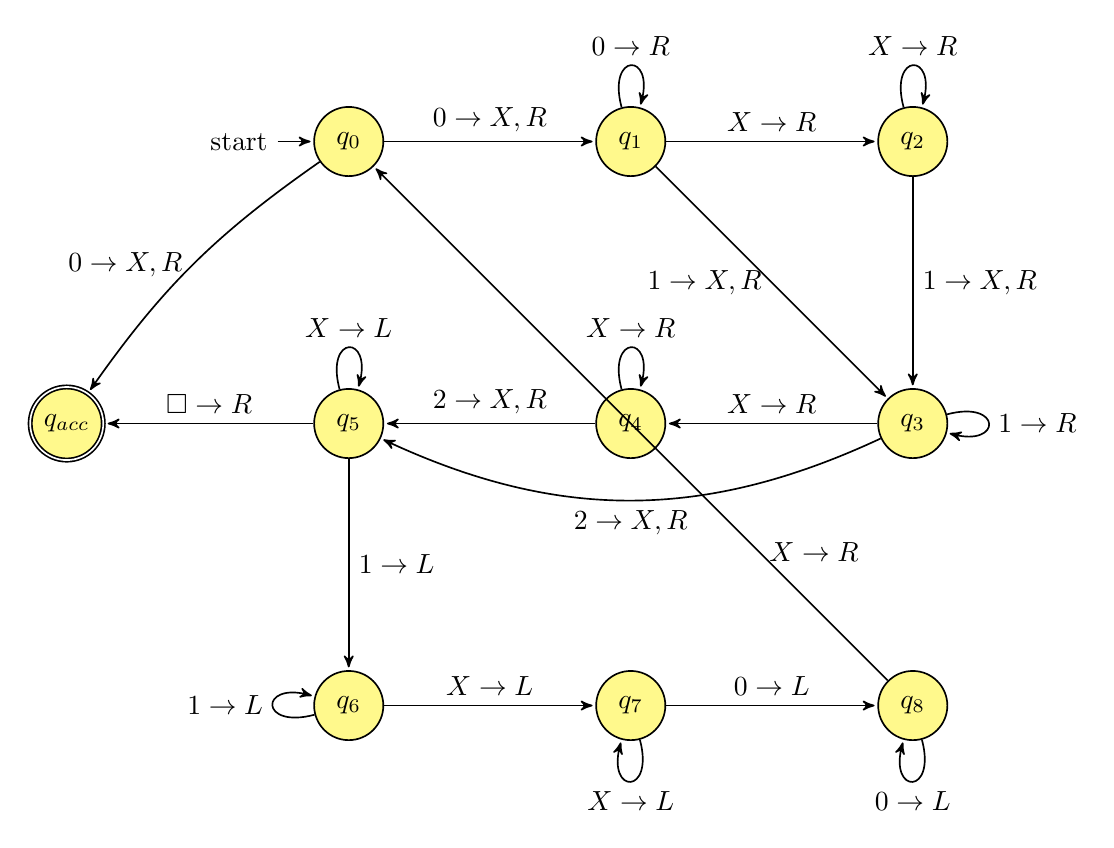
\begin{tikzpicture}[->,>=stealth',shorten >=1pt, auto, node distance=2cm, semithick]
          \tikzstyle{every state}=[text=black, fill=yellow!45]
          
          \node[initial,state] (q_0)          {$q_0$};
          \node[state] (q_1) [right of=q_0, xshift=45pt] {$q_1$};
          \node[state] (q_2) [right of=q_1, xshift=45pt] {$q_2$};
          \node[state] (q_3) [below of=q_2, yshift=-45pt] {$q_3$};
          \node[state] (q_4) [left of=q_3, xshift=-45pt] {$q_4$};
          \node[state] (q_5) [left of=q_4, xshift=-45pt] {$q_5$};
          \node[state] (q_6) [below of=q_5, yshift=-45pt] {$q_6$};
          \node[state] (q_7) [right of=q_6, xshift=45pt] {$q_7$};
          \node[state] (q_8) [right of=q_7, xshift=45pt] {$q_8$};
          \node[state, accepting] (q_{acc}) [left of=q_5, xshift=-45pt] {$q_{acc}$};
      
          \path (q_0) edge  [] node {$0 \to X, R$} (q_1)
                (q_0) edge  [left, bend right=10] node {$0 \to X, R$} (q_{acc})
                (q_1) edge  [loop above] node {$0 \to R$} (q_1)
                (q_1) edge  [] node {$X \to R$} (q_2)
                (q_1) edge  [left] node {$1 \to X, R$} (q_3)
                (q_2) edge  [loop above] node {$X \to R$} (q_2)
                (q_2) edge  [] node {$1 \to X, R$} (q_3)
                (q_3) edge  [loop right] node {$1 \to R$} (q_3)
                (q_3) edge  [bend left=25] node {$2 \to X, R$} (q_5)
                (q_3) edge  [above] node {$X \to R$} (q_4)
                (q_4) edge  [loop above] node {$X \to R$} (q_4)
                (q_4) edge  [above] node {$2 \to X, R$} (q_5)
                (q_5) edge  [loop above] node {$X \to L$} (q_5)
                (q_5) edge  [] node {$1 \to L$} (q_6)
                (q_5) edge  [above] node {$\square \to R$} (q_{acc})
                (q_6) edge  [loop left] node {$1 \to L$} (q_6)
                (q_6) edge  [] node {$X \to L$} (q_7)
                (q_7) edge  [loop below] node {$X \to L$} (q_7)
                (q_7) edge  [] node {$0 \to L$} (q_8)
                (q_8) edge  [loop below] node {$0 \to L$} (q_8)
                (q_8) edge  [right, near start] node {$X \to R$} (q_0)
                ;
          \end{tikzpicture}
      \end{center}

      \begin{center}
        \begin{tabular}{|c|c|c|c|c|}
          \hline
          \multicolumn{1}{|c}{\phantom{A}} & \multicolumn{1}{c}{$q_0\downarrow$} &  \multicolumn{3}{c|}{\phantom{A}}\\
          \hline
          $\square$ & $0$ & $1$  & $2$ & $\square $\\
          \hline
          \multicolumn{2}{|c}{\phantom{A}} & \multicolumn{1}{c}{$q_1\downarrow$} & \multicolumn{2}{c|}{\phantom{A}}\\
          \hline
          $\square$ & $X$ & $1$  & $2$ & $\square $\\
          \hline
          \multicolumn{3}{|c}{\phantom{A}} & \multicolumn{1}{c}{$q_3\downarrow$} & \multicolumn{1}{c|}{\phantom{A}}\\
          \hline
          $\square$ & $X$ & $X$  & $2$ & $\square $\\          
          \hline
          \multicolumn{4}{|c}{\phantom{A}} & \multicolumn{1}{c|}{$q_5\downarrow$}\\          
          \hline
          $\square$ & $X$ & $X$  & $X$ & $\square $\\         
          \hline
          \multicolumn{3}{|c}{\phantom{A}} & \multicolumn{1}{c}{$q_8\downarrow$} & \multicolumn{1}{c|}{\phantom{A}}\\          
          \hline
          $\square$ & $X$ & $X$  & $X$ & $\square $\\   
          \hline
          \multicolumn{2}{|c}{\phantom{A}} & \multicolumn{1}{c}{$q_8\downarrow$} & \multicolumn{2}{c|}{\phantom{A}}\\          
          \hline
          $\square$ & $X$ & $X$  & $X$ & $\square $\\   
          \hline
          \multicolumn{2}{|c}{$q_{8}\downarrow$} &  \multicolumn{3}{c|}{\phantom{A}}\\
          \hline
          $\square$ & $X$ & $X$  & $X$ & $\square $\\   
          \hline
          \multicolumn{1}{|c}{$q_{8}\downarrow$} &  \multicolumn{3}{c|}{\phantom{A}}\\
          \hline
          $\square$ & $X$ & $X$  & $X$ & $\square $\\   
          \hline
          \multicolumn{2}{|c}{$q_{acc}\downarrow$} &  \multicolumn{3}{c|}{\phantom{A}}\\
          \hline
          $\square$ & $X$ & $X$  & $X$ & $\square $\\   
          \hline
          \end{tabular}
      \end{center}
    \end{proof}
  \end{enumerate}
\end{homeworkProblem}

\newpage

\begin{homeworkProblem}
  For this question, consider the alphabet $\Sigma = \{0,1\}$.

  \begin{enumerate}[(a)]
  \item\gradeCorrect Give an example of a finite, nonempty language over $\Sigma$ and two different
  Turing machines that recognize it: one that is a decider and one that is not. A complete solution
  will include a precise definition for your example language, along with {\bf both} a state diagram
  and an implementation-level description of each Turing machines, along with a brief explanation of
  why each of them recognizes the language and why one is a decider and there other is not.

  \begin{proof}
    Consider the language $L = \{01\}$. Let $\Gamma = \{0, 1, \square\}$. Turing machines $M_1, M_2$
    are defined as below:
    \begin{center}
      \begin{multicols}{2}
          State diagram for $M_1$
      
          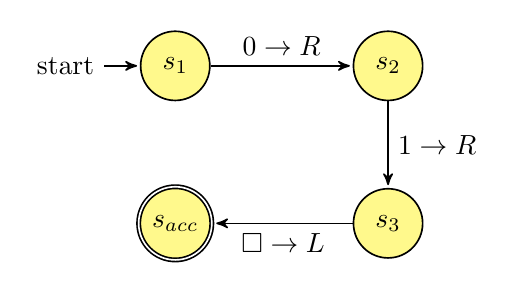
\begin{tikzpicture}[->,>=stealth',shorten >=1pt, auto, node distance=2cm, semithick]
          \tikzstyle{every state}=[text=black, fill=yellow!45]
          
          \node[initial, state] (s1)          {$s_1$};
          \node[state] (s2) [right of=s1, xshift=20pt]   {$s_2$};
          \node[state] (s3) [below of=s2]   {$s_3$};
          \node[state, accepting] (s4) [below of=s1]   {$s_{acc}$};
      
          \path (s1) edge  [] node {$0 \to R$} (s2)
                (s2) edge  [] node {$1 \to R$} (s3)
                (s3) edge  [] node {$\square \to L$} (s4)
          ;
          \end{tikzpicture}

          \columnbreak 
      
          State diagram for $M_2$
      
          \begin{tikzpicture}[->,>=stealth',shorten >=1pt, auto, node distance=2cm, semithick]
            \tikzstyle{every state}=[text=black, fill=yellow!45]
            
            \node[initial, state] (q1)          {$q_1$};
            \node[state] (q2) [right of=s1, xshift=20pt]   {$q_2$};
            \node[state] (q3) [below of=s2]   {$q_3$};
            \node[state, accepting] (q4) [below of=s1]   {$q_{acc}$};
        
            \path (q1) edge  [bend left=20] node {$0 \to R$} (q2)
                  (q2) edge  [bend left=20] node {$0, \square \to L$} (q1)
                  (q2) edge  [] node {$1 \to R$} (q3)
                  (q3) edge  [] node {$\square \to L$} (q4)
            ;
            \end{tikzpicture}
      \end{multicols}
      \end{center}
      \begin{multicols}{2}
        $M_1 = $ ``On input string $w$:
        \begin{enumerate}[1.]
          \item If the first tape symbol was $0$, move right. Otherwise, reject.
          \item If the next symbol is 1, move right. Otherwise, reject.
          \item If the next symbol is blank, move left and accept. Otherwise, reject.''
        \end{enumerate}

        \columnbreak 

        $M_2 = $ ``On input string $w$:
        \begin{enumerate}[1.]
          \item If the first tape symbol was $0$, move right. Otherwise, reject.
          \item If the second tape symbol was 1, move right and accept. Otherwise, move left and
          go to stage 1.
          \item If the next symbol is blank, move left and accept. Otherwise, reject.''
        \end{enumerate}
      \end{multicols}
      Since $M_1$ simply reads all the way right to check if the sequence is exactly $01$, $M_1$
      recognizes $L$ and is a decider. For $M_2$, if the input string $w = 01$, it would get sent to
      the accept state like in $M_1$. However, if $w \neq 01$, it would either get rejected at $q_1$
      or $q_3$, or get stuck in the loop of $q_1$ and $q_2$ forever. To see this, we may consider
      the string $0$. $0$ gets sent to $q_2$ sent back to $q_1$ as the second symbol is a blank. But
      then the machine head also goes back to the start of $w$ after reading the blank. It follows
      that the process restarts and loops forever, and thus $M_2$ is not a decider.
  \end{proof}

  \newpage

  \item\gradeCorrect True or false: There is a Turing machine that is not a decider that recognizes
  the empty set. A complete solution will include a witness Turing machine (given by state diagram
  or implementation-level description or high-level description) and a justification for why it's
  not a decider and why it does not accept any strings, or a complete and correct justification for
  why there is no such Turing machine.

  \begin{proof}
    True. Consider $T$ specified as below:
    \begin{center}
      State diagram of $T$

      \begin{tikzpicture}[->,>=stealth',shorten >=1pt, auto, node distance=2cm, semithick]
        \tikzstyle{every state}=[text=black, fill=yellow!45]
        
        \node[initial, state] (q1)          {$q_1$};
        \node[state] (q3) [right of=s1, xshift=20pt]     {$q_2$};
        \node[state, accepting] (q2) [right of=q3]   {$q_{acc}$};
    
        \path (q1) edge  [bend left=20] node {$0, 1, \square \to R$} (q3)
              (q3) edge  [bend left=20] node {$0, 1, \square \to L$} (q1)
        ;
        \end{tikzpicture}
    \end{center}
    Let $w \in \Sigma^*$. $w$ gets sent to $q_2$ and sent back to $q_1$. But then the machine head
    also goes back to the starting point, and thus $w$ ends up in a loop. Hence, $T$ is not a
    decider but recognizes the empty set.
  \end{proof}

  \item\gradeCorrect True or false: There is a Turing machine that is not a decider that recognizes
  the set of all string $\Sigma^*$.  A complete solution will include a witness Turing machine
  (given by state diagram or implementation-level description or high-level description) and a
  justification for why it's not a decider and why it accept each string over $\{0,1\}$, or a
  complete and correct justification for why there is no such Turing machine.

  \begin{proof}
    False. Note that Turing machines halt on acception. Since every string over $\Sigma$ gets
    accepted, the machine would halt on any input. 
  \end{proof}
  \end{enumerate}
\end{homeworkProblem}

\newpage

\begin{homeworkProblem}
  Suppose $M$ is a Turing machine over the alphabet $\{0,1\}$. Let $s_1, s_2, \ldots$ be a list of
  all strings in $\{0,1\}^*$ in string (shortlex) order. We define a new Turing machine by giving
  its high-level description as follows: 
  \begin{align*}
    M_{new} &= ``\text{On input }w:\\
      &\text{1.For $n = 1, 2, \ldots$}\\
      &\text{2.~~~For $j = 1, 2, \ldots n$} \\
      &\text{3.~~~For $k = 1, 2, \ldots, n$} \\
      &\text{4.~~~~~~Run the computation of $M$ on $s_jws_k$}\\
      &\text{5.~~~~~~If it accepts, accept.}\\
      &\text{6.~~~~~~If it rejects, go to the next iteration of the loop"}\\
  \end{align*}

  Recall the definitions we have: For languages $L_1, L_2$ over the alphabet $\Sigma = \{0,1\}$, we
  have the associated sets of strings
  \[
    SUBSTRING(L_1) = \{ w \in \Sigma^* ~|~ \text{there exist } a,b \in \Sigma^* \text{ such that } awb \in L_1\}
  \]
  and 
  \[
    L_1 \circ L_2 = \{ w \in \Sigma^* ~|~ w = uv \text{ for some strings } u \in L_1 \text{ and } v \in L_2 \}
  \]
  We say that self-set-wise concatenation of the set $L_1$ is $L_1 \circ L_1$.

  \begin{enumerate}[(a)]
  \item \gradeComplete Prove that this Turing machine construction {\bf cannot} be used to prove
  that the class of decidable languages over $\{0,1\}$ is closed under {\bf either} of the above
  operations ($SUBSTRING$ or self-set-wise concatenation). A complete answer will give a
  counterexample or general description why the construction doesn't work for both operations.
  \begin{proof}
    Consider a Turing machine $M_1$ that recognizes the language $L_1 = \{00\}$. and let $M_1'$ be
    the resulting construction. Note that $L_1$ is finite, so it is Turing decidable. Let $w = 1$.
    Since for all $s_j, s_k \in \{0, 1\}^*$, $s_jws_k$ is never recognized by $M$, the loop $M_1'$
    never ends. It follows that $M_1'$ does neither decides $SUBSTRING(L_1)$ nor $L_1 \circ L_1$.
  \end{proof}
  \item \gradeCorrect Prove that this Turing machine construction cannot be used to prove that the
  class of recognizable languages over $\{0,1\}$ is closed under the $SUBSTRING$ set operation. In
  particular, give a counterexample of a specific language $L_1$ and Turing machine $M_1$
  recognizing it where $M_{new}$ does not recognize $SUBSTRING(L_1)$.
  \begin{proof}
    Consider $M_2$ defined in problem 2 part (a). Let $w = 0$. We know $L(M_2) = \{01\}$, so $w$ is
    in $SUBSTRING(L(M_2))$. However, since $M_{new}$ enumerates the strings in shortlex order, $0$
    would get inputted to $M$ before $01$ does. Thus, $01$ would not get read in finite time, as $M$
    loops on $0$. It follows that $w$ would not get accepted by $M_{new}$, and thus $M_{new}$ does
    not recognize $SUBSTRING(L(M_2))$.
  \end{proof}
  \newpage
  \item \gradeComplete Define a new construction by slightly modifiying this one that can be used to
  prove  that the class of recognizable languages over $\{0,1\}$ is closed under $SUBSTRING$.
  Justify that your construction works. The proof of correctness for the closure claim can be
  structured like: ``Let $L_1 $ be a recognizable language over $\{0,1\}$ and assume we are given a
  Turing machine $M_1$ so that $L(M_1) = L_1$. Consider the new Turing machine $M_{new}$ defined
  above. We will show that $L(M_{new}) = SUBSTRING(L_1) $... {\it complete the proof by proving
  subset inclusion in two directions, by tracing the relevant Turing machine computations}''
  \begin{proof}
    Consider the construction 
    \begin{align*}
      M_{new} &= ``\text{On input }w:\\
        &\text{1.For $n = 1, 2, \ldots$}\\
        &\text{2.~~~For $j = 1, 2, \ldots n$} \\
        &\text{3.~~~For $k = 1, 2, \ldots, n$} \\
        &\text{4.~~~~~~Run the computation of $M$ on $s_jws_k$ for at most $n$ steps}\\
        &\text{5.~~~~~~If it accepts, accept.}\\
        &\text{6.~~~~~~If it rejects, go to the next iteration of the loop"}\\
    \end{align*}

    Let $L_1 $ be a recognizable language over $\{0,1\}$ and assume we are given a Turing machine
    $M_1$ so that $L(M_1) = L_1$. Consider the new Turing machine $M_{new}$ defined above. We will
    show that $L(M_{new}) = SUBSTRING(L_1)$. Let $w \in L(M_{new})$. Since $w$ is accepted by
    $M_{new}$, $s_jws_k$ is accepted by $M$, for some $s_j, s_k$. Hence, $w \in SUBSTRING(L_1)$. 

    we now suppose $w \in SUBSTRING(L_1)$. Then, there exsits $s_j, s_k$ such that $s_jws_k \in
    L_1$. Since $M_{new}$ only run each subloops in finite time, the subloops in $M_{new}$ would
    eventually reach $i, k$, and thus it would eventually run $s_jws_k$ on $M$, which would then get
   accepted. Hence, $w \in L(M_{new})$. 
  \end{proof}
  \end{enumerate}
\end{homeworkProblem}

\newpage

\begin{homeworkProblem}
  Recall the definitions of some example computational problems from class

  \hspace{-7.5pt}
  \begin{tabular}{|lcl|}
    \hline
    \multicolumn{3}{|l|}{{\bf  Acceptance problem} } \\
    & & \\
    \ldots for DFA & $A_{DFA}$ & $\{ \langle B,w \rangle \mid  \text{$B$ is a  DFA that accepts input 
    string $w$}\}$ \\
    \ldots for NFA & $A_{NFA}$ & $\{ \langle B,w \rangle \mid  \text{$B$ is a  NFA that accepts input 
    string $w$}\}$ \\
    \ldots for regular expressions & $A_{REX}$ & $\{ \langle R,w \rangle \mid  \text{$R$ is a  regular
    expression that generates input string $w$}\}$ \\
    \ldots for CFG & $A_{CFG}$ & $\{ \langle G,w \rangle \mid  \text{$G$ is a context-free grammar 
    that generates input string $w$}\}$ \\
    \ldots for PDA & $A_{PDA}$ & $\{ \langle B,w \rangle \mid  \text{$B$ is a PDA that accepts input string $w$}\}$ \\
    & & \\
    \hline
    \multicolumn{3}{|l|}{{\bf Language emptiness  testing} } \\
    & & \\
    \ldots for DFA & $E_{DFA}$ & $\{ \langle A \rangle \mid  \text{$A$ is a  DFA and  $L(A) = \emptyset$\}}$ \\
    \ldots for NFA & $E_{NFA}$ & $\{ \langle A\rangle \mid  \text{$A$ is a NFA and  $L(A) = \emptyset$\}}$ \\
    \ldots for regular expressions & $E_{REX}$ & $\{ \langle R \rangle \mid  \text{$R$ is a  regular
    expression and  $L(R) = \emptyset$\}}$ \\
    \ldots for CFG & $E_{CFG}$ & $\{ \langle G \rangle \mid  \text{$G$ is a context-free grammar 
    and  $L(G) = \emptyset$\}}$ \\
    \ldots for PDA & $E_{PDA}$ & $\{ \langle A \rangle \mid  \text{$A$ is a PDA and  $L(A) = \emptyset$\}}$ \\
    & & \\
    \hline
    \multicolumn{3}{|l|}{{\bf Language equality testing} } \\
    & & \\
    \ldots for DFA & $EQ_{DFA}$ & $\{ \langle A, B \rangle \mid  \text{$A$ and $B$ are DFAs and  $L(A) =L(B)$\}}$\\
    \ldots for NFA & $EQ_{NFA}$ & $\{ \langle A, B \rangle \mid  \text{$A$ and $B$ are NFAs and  $L(A) =L(B)$\}}$\\
    \ldots for regular expressions & $EQ_{REX}$ & $\{ \langle R, R' \rangle \mid  \text{$R$ and $R'$ are regular
    expressions and  $L(R) =L(R')$\}}$\\
    \ldots for CFG & $EQ_{CFG}$ & $\{ \langle G, G' \rangle \mid  \text{$G$ and $G'$ are CFGs and  $L(G) =L(G')$\}}$ \\
    \ldots for PDA & $EQ_{PDA}$ & $\{ \langle A, B \rangle \mid  \text{$A$ and $B$ are PDAs and  $L(A) =L(B)$\}}$ \\
    \hline
  \end{tabular}
  
  \begin{enumerate}[(a)]
    \item \gradeComplete Pick five of the computational problems above and give 
    examples (preferably different from the ones we talked about in class) of strings that are
    in each of the corresponding languages. Remember to use the 
    notation $\langle \cdots \rangle$ to denote the string encoding of relevant objects.
    {\it Extension, not for credit:} Explain why it's hard to write a specific string of 
    $0$s and $1$s and make a claim about membership in one of these sets.
    \begin{proof}
      Let $M_1$ a DFA, $M_2$ be an NFA, $R$ be a regular expression, $G$ be a CFG, $P$ be a PDA.
      Then, $\langle M_1, M_1 \rangle \in EQ_{DFA}$, $\langle M_2, M_2 \rangle \in EQ_{NFA}$,
      $\langle R, R \rangle \in EQ_{REX}$, $\langle G, G \rangle \in EQ_{CFG}$, and $\langle P, P
      \rangle \in EQ_{PDA}$.
    \end{proof}
    \item \gradeComplete Computational problems can also be defined about Turing machines.
    Consider the two high-level descriptions of Turing machines below.
    Reverse-engineer them to define the computational problem that is being
    recognized, where $L(M_{DFA})$ is the language corresponding to this computational
    problem about DFA and $L(M_{TM})$ is the language corresponding to this computational
    problem about Turing machines. {\it Hint}: the computational problem is not acceptance,
    language emptiness, or language equality (but is related to one of them).

    Let $s_1, s_2, \ldots$ be a list of all strings in 
    $\{0,1\}^*$ in string (shortlex) order. Consider the following Turing machines
    \begin{align*}
        M_{DFA} &= ``\text{On input $\langle D \rangle$ where $D$ is a DFA}:\\
          &\text{1. for $i=1, 2, 3, \ldots$} \\
          &\text{2.~~~ Run $D$ on $s_i$} \\
          &\text{3.~~~~If it accepts, accept.}\\
          &\text{4.~~~~If it rejects, go to the next iteration of the loop"}\\
      \end{align*}
      and
      \begin{align*}
        M_{TM} &= ``\text{On input $\langle T \rangle$ where $T$ is a Turing machine}:\\
          &\text{1. for $i=1, 2, 3, \ldots$} \\
          &\text{2.~~~ Run $T$ for $i$ steps on each input $s_1, s_2, \ldots, s_i$ in turn} \\
          &\text{3.~~~~If $T$ has accepted any of these, accept.}\\
          &\text{4.~~~~Otherwise, go to the next iteration of the loop"}\\
      \end{align*}
      \begin{proof}
        $M_{DFA}$ recognizes any $D$ such that $L(D)$ is nonempty, and thus the computational
        problem can be defined as $\overline{E_{DFA}}$, the complement of $E_{DFA}$. 

        On the other hand, $M_{TM}$ recognizes Turing machine $T$ such that $L(T) \cap S \neq
        \emptyset$, for a fixed language $S = \{s_i \mid i \in \N\}$. Hence, we may define the
        computation problem as $\{\langle T \rangle \mid T \text{ is a Turing machine and } L(T)
        \cap \{s_i \mid i \in \N\} \neq \emptyset\}$
      \end{proof}
  \end{enumerate}
\end{homeworkProblem}
\end{document}